%!Tex Root = ../main.tex
% ./Packete.tex
% ./Design.tex
% ./Deklarationen.tex
% ./Vorbereitung.tex
% ./Aufgabe1.tex
% ./Aufgabe3.tex
% ./Aufgabe4.tex
% ./Bonus.tex

\section{Aufgabe 2}

\setcounter{exercise}{1}

\begin{frame}[allowframebreaks]{Aufgabe \thesection}{XYZ}
  \begin{solutionnoinc}
    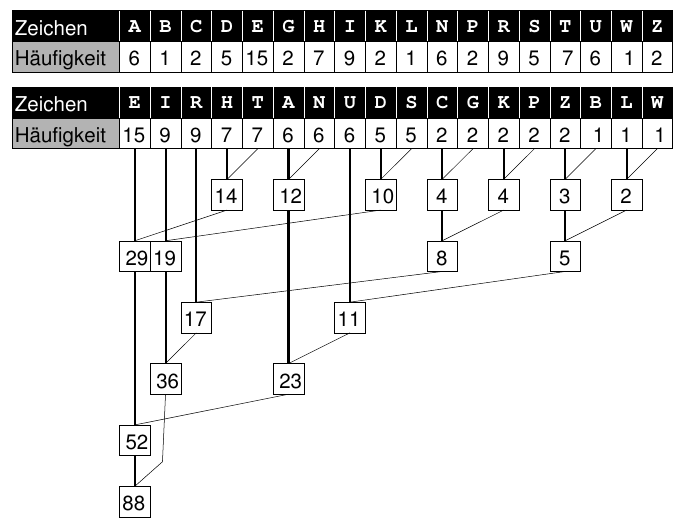
\includegraphics[width=0.3\textwidth, center]{./figures/huffman_code.png}
  \end{solutionnoinc}
  \begin{Sidenote}
    \begin{itemize}
      \item die Codewörter müssen ausgehend von der Wurzel zu den Blättern aufgebaut werden, sonst ergibt sich kein Präfixcode
    \end{itemize}
  \end{Sidenote}
  \begin{solution}
    \definecolor{VeniceBlue}{rgb}{0.043,0.392,0.627}
    \definecolor{Ivory}{rgb}{1,1,1}
    \resizebox{\textwidth}{!}{
      \begin{minipage}[t]{26cm}
        \begin{table}
          \centering
          \begin{tblr}{
              cells = {Ivory},
              column{1} = {PrimaryColor,fg=white},
            }
            Zeichen &  E  &  I  &  R  &   H  &  T   &   A  &  N   &   U  &  D   &  S   &   C   &   G   &   K   &   P   &   Z    &    B   &    L   &  W  \\
            Code    & 000 & 100 & 110 & 0010 & 0011 & 0100 & 0101 & 0110 & 1010 & 1011 & 11100 & 11101 & 11110 & 11111 & 011100 & 011101 & 011110 & 011111
          \end{tblr}
        \end{table}
      \end{minipage}
    }
  \end{solution}
  \begin{Sidenote}
    \begin{itemize}
      \item Ein Präfixcode ist ein Code, bei dem kein Codewort Präfix eines anderen Codewortes ist. 
      \item Z.B. wäre ein Code mit den Codewörtern $a = 10$, $b = 101$ kein Code, da man beim Dekodieren einer Nachricht beim
      Lesen von $10$ nicht weiß, ob damit $a$ oder, bei einer nachfolgenden $1$, das Wort $b$ gemeint ist. 
      \item Einen Präfixcode kann man also \enquote{online} dekodieren, d.h. man liest Zeichen für Zeichen und bei einem Matching mit einem Wort im Wörterbuch hat man das ursprüngliche Wort gefunden.
    \end{itemize}
  \end{Sidenote}
  \begin{solution}
    \begin{itemize}
      \item \alert{Dekodierung:} TI IST KLASSE
        \[
          \underbrace{0011}_{T}\;\underbrace{100}_{I}\;\underbrace{100}_{I}\;\underbrace{1011}_{S}\;\underbrace{0011}_{T}\;\underbrace{11110}_{K}\;\underbrace{011110}_{L}\;\underbrace{0100}_{A}\;\underbrace{1011}_{S}\;\underbrace{1011}_{S}\;\underbrace{000}_{E}
        \]
      \item \alert{Mögliches Problem:} Codierung von Blättern hin zur Wurzel $\rightarrow$ \textit{kein Präfix-Code}, Dekodierung nicht möglich (s.o.)
    \end{itemize}
  \end{solution}
  \begin{solution}
    \begin{itemize}
      \item Damit andere die Nachricht dekodieren (d.h. lesen) können, muss man natürlich auch das Wörterbuch (d.h. die generierte Code-Tabelle) mitliefern. 
      \item Da damit jedem, der die kodierte Nachricht erhält, auch die Dekodierungstabelle zugänglich ist, kann natürlich jeder die Nachricht dekodieren. D.h. die kodierte Nachricht genügt keinen kryptologischen Ansprüchen. 
      \item Was man allerdings erreicht hat, ist eine Datenkomprimierung (bei großen Texten).
    \end{itemize}
  \end{solution}
\end{frame}
